\section{Analyse de donn\'ees}

A pr\'esent, nous pouvons nous concentrer sur l'analyse des donn\'ees dans le but de caract\'eriser l'OM.

En vous basant sur les donn\'ees, vous devrez calculer:
\begin{center}
\fbox{
\begin{minipage}{0.75\textwidth}
\textbf{Dispositif muon :}
\begin{itemize}
\item le gain $G$ de l'OM,
\item la r\'esolution $\sigma_\mathrm{G}$ de l'OM,
\item le nombre moyen de photo-\'electrons $\langle n_{\mathrm{pe}}\rangle$ produit par trigger dans l'OM.
\end{itemize}
\end{minipage}
}
\end{center}

\ifthenelse{\boolean{showAdditional}}{
\begin{additional}
\textbf{Validation de la procedure d'adjustement:}\\
\includegraphics[width=\textwidth]{exampleAnalysis/LLFit_MC.pdf}\\
\textbf{Dispositif electrons:}\\
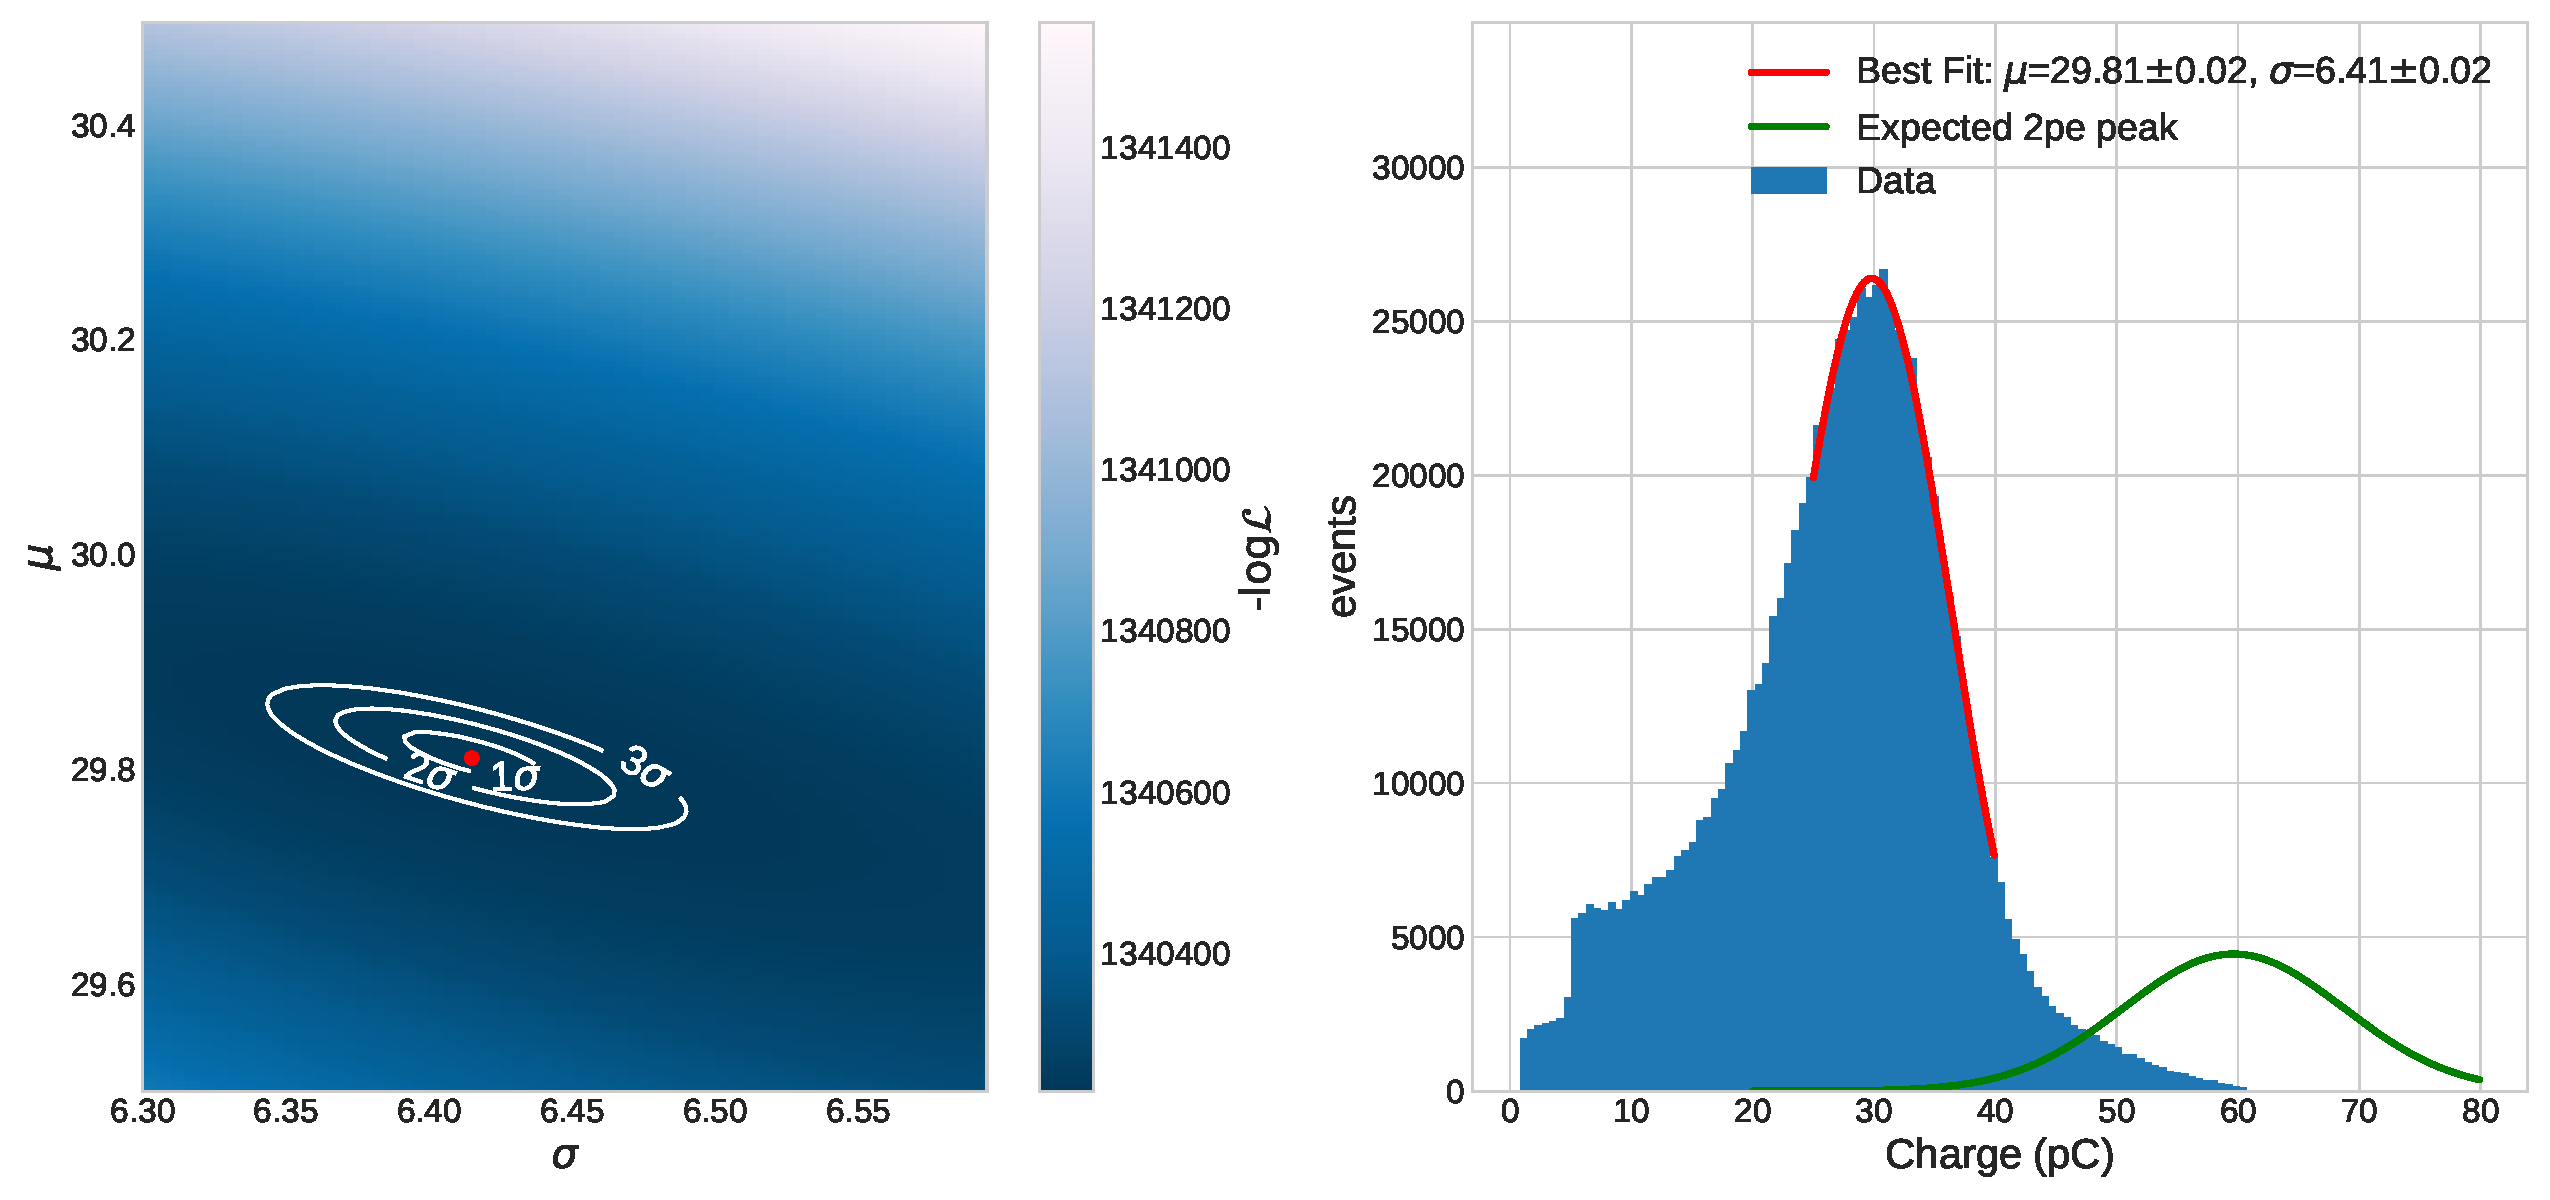
\includegraphics[width=\textwidth]{exampleAnalysis/LLFit_Data_1pe.pdf}\\
\begin{align}
G &= \mu_{\text{best}}/e = 185963 \\
\sigma_G &= \sigma_{\text{best}} / \mu_{\text{best}} = 21.52\%\\
\langle n_{\mathrm{pe}}\rangle &= \text{n.a.}
\end{align}
{\centering
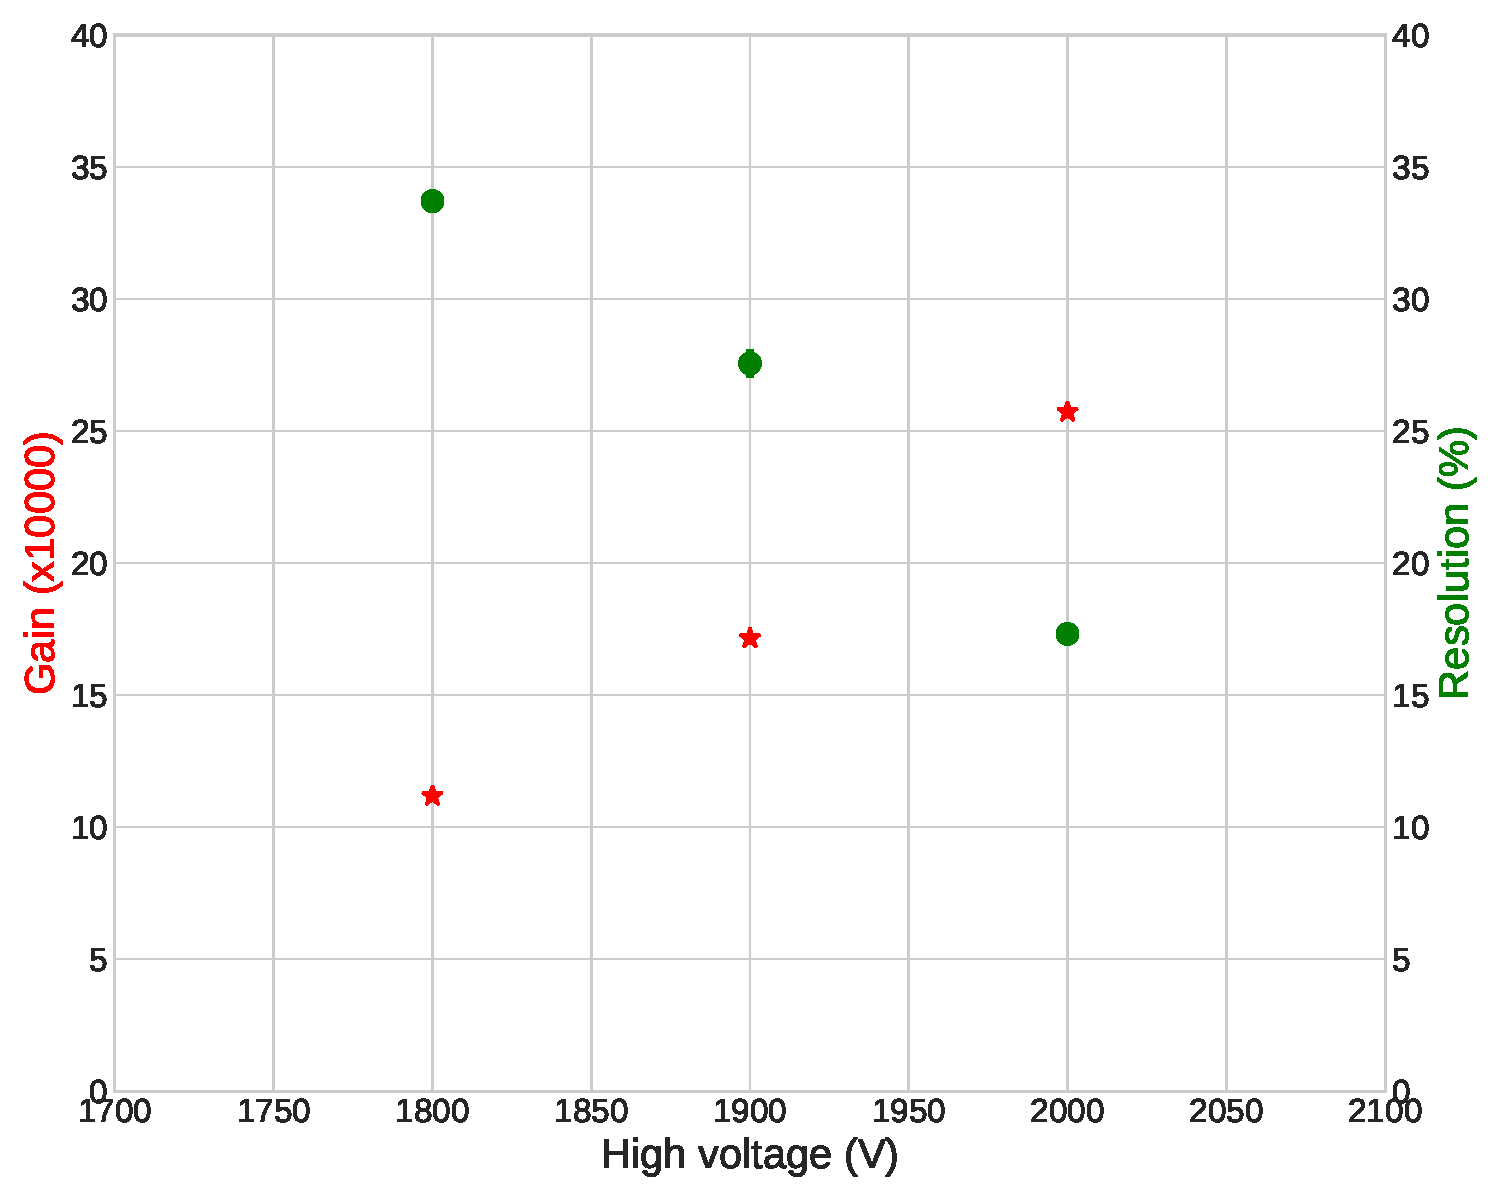
\includegraphics[width=0.7\textwidth]{exampleAnalysis/Gain_Resolution_HV.pdf}\\}
\textbf{Dispositif muons:}\\
\end{additional}
}

\pagebreak